\section{Noise Attenuation Measurements}

\subsection{Purpose}

The purpose of this experience is to determine the SNR needed to understand speech in a noisy office environment. 

\subsection{AAU number list}
The materials used for the experiments is noted in table \ref{tab:UsedEquipmentListningAttenuation}. The items are paired with a number which corresponds with the same number on figure \ref{fig:AttenuationSetup}.

\begin{table}[h]
	\centering
	
	\begin{tabular}{ c c c } \toprule
		{Item} & {Description} & {AAU-no}. \\ \bottomrule 
		1      	&  USB keyboard							& NaN		\\
		2      	&  Beyerdynamic DT770pro				& 2037-18	\\
		3      	&  Soundcard RME Fireface 802           & 86838		\\
		4      	&  Computer	running Simulink			& NaN		\\  
		5		&  HATS with SPL-meter				& 2150-04	\\
		6      	&  Genelec speaker A					& 33984		\\
		7      	&  Genelec speaker B					& 33989		\\
		8      	&  Genelec speaker C					& 33987		\\
		9      	&  Genelec speaker D					& 33990		\\ \bottomrule 
	\end{tabular}
	\caption{Equipment used in the experiment}
	\label{tab:UsedEquipmentListningAttenuation}
\end{table}



\subsubsection{Diagram}

\begin{table} [h]
	\centering
	\begin{tabular}{c c} \toprule
		\centering
		Height of:			 			& Measurement [cm] 	\\ \bottomrule
		Speakers					  	& 100				\\
		The ear of participant			& 110				\\ 
		Table							& 90				\\ \bottomrule 
	\end{tabular}
	\caption{Height of setup. Speakers are placed with tweeters on the bottom.}
	\label{Tab:NoiseAttenuationDimensions}
\end{table}

\begin{figure}[H]
	\centering
	\includegraphics[width=12cm]{AttenuationExperiment/setup}
	\caption{Setup of Noise attenuation experiment}
	\label{Fig:NoiseAttenuationExperimet}
\end{figure}


\subsubsection{Settings/Description}
Our setting aims at reproducing an office sound field. We chose to produce the sound field with 4 speakers. 
The idea is to reproduce a real life situation in an office. Speech and office background noise is played on four speakers. Speaker C and D in figure \ref{Fig:NoiseAttenuationExperimet} play speech signals. Speaker A and B play ambient office noise. The listener who is seated in front of speakers will wear a pair of headphones playing speech. This setup emulates a phone call in a noisy office. The test will run six times with each participant. The first test is a "trial" and will not be used in data analysis. The following three will run at "high level" according to table \ref{tab:SPLCalibration}. The last two test will run at "low level". 

The participant has control of a slider using a keyboard adjusting the sound level of the 4 speakers in the room, allowing them to attenuate the background noise. their role will be to find the noise level where they can understand the speech on the headset, without being disturbed significantly by the noisy environment. The slider has a range from 0 dB to -40 dB with steps of 0.4dB. 

The Sound pressure levels of the sources are calibrated at the position of the listener. The calibration is made with all gain settings on the computer and in Simulink set to 0dB (including the slider). The HATS is placed at the listening position and the built in SPL-meter is used to find the levels of the noise from the two sets of speakers individually and in combination. 
The same method is used is used to find the SPL of the sound in the headphones. The headphones are placed over the ears of "Valdemar" and a readout is made. The levels are equal to the values below.
\begin{table} [H]
\centering
	\begin{tabular}{c c}											\toprule
		Sound source				& 	SPL [dBre20\micro Pa]	\\ 	\bottomrule
		Speaker C \& D				& 	72.5					\\
		Speaker A \& B				&	70						\\
		All speakers				&	74						\\
		Headphone high level		&	68						\\ 	
		Headphone low level			&	58						\\	\bottomrule
	\end{tabular}
	\caption{SPL calibration table - tolerance $\pm$2.5dB.}
	\label{tab:SPLCalibration}
\end{table}   



\subsubsection{Picture and setup}

\begin{figure}[H]
\centering
  \begin{subfigure}[b]{0.5\textwidth}
  \centering
	\tikzsetnextfilename{AttenuationSetup}
	
\definecolor{cffffff}{RGB}{255,255,255}

\resizebox {0.4\columnwidth} {!} {
\begin{tikzpicture}[y=0.80pt, x=0.80pt, yscale=-1.000000, xscale=1.000000, inner sep=0pt, outer sep=0pt]
\begin{scope}% layer1
  % text3396
  \path[fill=black,line join=miter,line cap=butt,line width=0.800pt]
    (242.8571,610.2194) node[above right] (text3396) {};

  % rect5654
  \path[draw=black,fill=cffffff,opacity=0.980,miter limit=4.00,line
    width=0.837pt,rounded corners=0.0000cm] (0.0000,492.3622) rectangle
    (460.0000,1052.3622);

  % path5656
  \path[draw=black,dash pattern=on 2.40pt off 0.80pt,line join=miter,line
    cap=butt,miter limit=4.00,even odd rule,line width=0.800pt] (0.0000,482.3622)
    .. controls (460.0000,482.3622) and (460.0000,482.3622) ..
    (460.0000,482.3622);

  % path6121
  \path[draw=black,dash pattern=on 2.40pt off 0.80pt,line join=miter,line
    cap=butt,miter limit=4.00,even odd rule,line width=0.800pt]
    (470.0000,1052.3622) -- (470.0000,492.3622);

  % rect6329
  \path[draw=black,fill=cffffff,opacity=0.980,miter limit=4.00,line
    width=0.800pt,rounded corners=0.0000cm] (220.1005,972.3622) rectangle
    (260.1005,1012.3622);

  % rect6329-8
  \path[draw=black,fill=cffffff,opacity=0.980,miter limit=4.00,line
    width=0.800pt,rounded corners=0.0000cm] (50.3174,692.3748) rectangle
    (90.3174,732.3748);

  % rect6329-8-5
  \path[draw=black,fill=cffffff,opacity=0.980,miter limit=4.00,line
    width=0.800pt,rounded corners=0.0000cm] (370.6172,692.3992) rectangle
    (410.6172,732.3992);

  % rect6329-8-1
  \path[draw=black,fill=cffffff,opacity=0.980,miter limit=4.00,line
    width=0.800pt,rounded corners=0.0000cm] (220.0700,651.8595) rectangle
    (260.0700,691.8595);

  % path6381
  \path[draw=black,fill=cffffff,opacity=0.980,miter limit=4.00,line width=0.800pt]
    (239.6594,819.1820) circle (0.4233cm);

  % path6695
  \path[draw=black,dash pattern=on 2.40pt off 0.80pt,line join=miter,line
    cap=butt,miter limit=4.00,even odd rule,line width=0.800pt] (50.0000,732.3622)
    -- (50.0000,1052.3622);

  % path6697
  \path[draw=black,dash pattern=on 2.40pt off 0.80pt,line join=miter,line
    cap=butt,miter limit=4.00,even odd rule,line width=0.800pt] (0.0000,692.3622)
    -- (220.0000,692.3622) -- (220.0000,1052.3622);

  % path6699
  \path[draw=black,dash pattern=on 2.40pt off 0.80pt,line join=miter,line
    cap=butt,miter limit=4.00,even odd rule,line width=0.800pt]
    (370.0000,732.3622) -- (0.0000,732.3622);

  % text4186
  \path[cm={{0.0,-1.0,1.0,0.0,(0.0,0.0)}},fill=black,line join=miter,line
    cap=butt,line width=0.800pt] (-1049.0592,215.0796) node[above right,rotate=90]
    (text4186) {16 cm};

  % text4186-3
  \path[cm={{0.0,-1.0,1.0,0.0,(0.0,0.0)}},fill=black,line join=miter,line
    cap=butt,line width=0.800pt] (-926.5287,234.3933) node[above right,rotate=90]
    (text4186-3) {15 cm};

  % text4186-1
  \path[fill=black,line join=miter,line cap=butt,line width=0.800pt]
    (252.8320,728.8373) node[above right] (text4186-1) {14 cm};

  % text4186-2
  \path[fill=black,line join=miter,line cap=butt,line width=0.800pt]
    (89.1852,688.5429) node[above right] (text4186-2) {13 cm};

  % text4186-4
  \path[fill=black,line join=miter,line cap=butt,line width=0.800pt]
    (1.3101,746.2242) node[above right] (text4186-4) {12 cm};

  % text4186-0
  \path[cm={{0.0,-1.0,1.0,0.0,(0.0,0.0)}},fill=black,line join=miter,line
    cap=butt,line width=0.800pt] (-914.2587,63.6862) node[above right,rotate=90]
    (text4186-0) {11 cm};

  % text4186-3-8
  \path[cm={{0.0,-1.0,1.0,0.0,(0.0,0.0)}},fill=black,line join=miter,line
    cap=butt,line width=0.800pt] (-781.0693,486.7263) node[above right,rotate=90]
    (text4186-3-8) {10 cm};

  % text4186-3-6
  \path[fill=black,line join=miter,line cap=butt,line width=0.800pt]
    (203.8091,475.7764) node[above right] (text4186-3-6) {17 cm};

  % text4186-2-1
  \path[fill=black,line join=miter,line cap=butt,line width=0.800pt]
    (63.7294,718.4424) node[above right] (text4186-2-1) {A};

  % text4186-2-1-2
  \path[fill=black,line join=miter,line cap=butt,line width=0.800pt]
    (232.8284,677.5307) node[above right] (text4186-2-1-2) {B};

  % text4186-2-1-9
  \path[fill=black,line join=miter,line cap=butt,line width=0.800pt]
    (385.7573,717.3333) node[above right] (text4186-2-1-9) {C};

  % text4186-2-1-6
  \path[fill=black,line join=miter,line cap=butt,line width=0.800pt]
    (233.8228,997.7496) node[above right] (text4186-2-1-6) {D};

  % text4326
  \path[fill=black,line join=miter,line cap=butt,line width=0.800pt]
    (233.0000,826.8622) node[above right] (text4326) {1};

\end{scope}

\end{tikzpicture}}


	\caption{Schematic overview of the setup}
	\label{fig:AttenuationSetup}
  \end{subfigure}\qquad
    \begin{subfigure}[b]{0.4\textwidth}
    \includegraphics[width=\textwidth]{AttenuationExperiment/AttenuationSetupBack}
    \caption{Setup from the back}
    \label{fig:SetupFront}
\vspace{2ex}
    \includegraphics[width=\textwidth]{AttenuationExperiment/AttenuationSetupFront}
    \caption{Setup from the front}
    \label{fig:SetupBack}
  \end{subfigure}
  \caption{Picture of setup and the specific schematic}
\end{figure}


\subsection{Procedure}

\begin{enumerate}
	\item Place the participant in the listening position.
	\item Instruct the participant as described in section \ref{subsubsec:attenuationInformation}.
	\item The participant will put on headphones and adjust them to fit their head.
	\item Run Simulink \path{XX.mat} with testnumber equal to 1 and gain slider at 0 dB.
	\item The participant selects noise level using arrow keys on the keyboard.
	\item Operator notes the attenuation value chosen by the participant.
	\item Repeat step 4-6, with testnumber equal to 2 through 6.
\end{enumerate}

\subsubsection{Information}\label{subsubsec:attenuationInformation}
The participant should read the instructions themselves to minimize how interaction between operator and participant influences the results. It is of course possible to ask questions.   
Ask the participant to read the following printout:

\textit{Imagine that you are sitting in a busy office environment. You are trying to hear a person speaking to you in a pair of headphones. \\\\
After reading this text, please put on and adjust the headphones.\\\\
The speakers around you will play background noise and speech. The headphones will play a recorded voice. Your task is to adjust the volume of the speakers using the left and right arrow keys on the keyboard in front of you. The speaker volume will start at maximum level. \\
When you have found the maximum level at which the noise is not a disturbance to your understanding of the voice, wait a moment to confirm your selection. When you are certain of your choice notify the operator. 
The test will be repeated seven times with different voices. \\\\
The definition of the noise being a "disturbance to your understanding of the understanding of the voice" is that you should be able to distinguish the voice from the noise without much concentration. This does not necessarily mean that the noise should be inaudible. Again imagine the situation, where you want to hear a person telling you something in a headphone in a busy office.\\\\ 
If you are in doubt of anything please ask the operator before fitting the headphones or if necessary during the first test.}

% Why is this repeated in a different wording? In this section??
%\begin{enumerate}
%\item We will play on the speakers office environnement sounds and speech. 
%\item The listener will put the headphones on.
%\item We will play in the headphones the file "speech1"
%\item The listener will then adjust the sound level on the speakers thank to a keyboard operating a matlab script. The listener will then stop adjusting the level when he reachs a level of "non disturbance"
%\item The listener will then adjust the sound level on the speakers thank to a keyboard operating a matlab script. The listener will then stop adjusting the level when he reachs a level of "non disturbance" "Speech understanding"
%\item We note the two attenuation levels for the given recording
%\item We change the file being played in the headphone and repeat the experience from 3.
%\end{enumerate}

\subsection{Data Extraction}
Results will be extracted manually from Simulink to a table during the test.
For each test the following table will be filled \\
\begin{table}[H]
\centering
	\begin{tabular}{c  c} \toprule
		experiment number & dB noise sources not disturbing  \\ \bottomrule
		1	&   \\
		2	&	\\
		3	&	\\
		4	&	\\
		5	&	\\
		6	&	\\ \bottomrule
	\end{tabular}
	\caption{Results of a listening test}
	\label{tab:ListeningRes}
\end{table}

\subsection{Analysis}
Compute statistics in Excel in order to find the overall attenuation needed by the system to be efficient.

\subsection{Changes after Pilot test}
During the pilot the instructions were shorter and read aloud. This resulted in a lot of questions after the instruction was given. For the main test it has therefore been chosen to make a written instruction, so people could reread sections if needed. This resulted in fewer questions after the instruction. \\
The amount of tests per participant was increased, which allowed testing at more than one gain setting in the headphones. \\
Small corrections to the physical setup was also made. 

\subsection{Notes from operator}
\begin{itemize}
\item The written instruction might be too long, participants felt the need to excuse their slow reading.
\item participants suggesting deleting the first experiment due to misunderstanding of the instruction. This choice had already been made, maybe it would be beneficial to tell the participants that the first experiment was a dummy. 
\end{itemize}

\subsection{Error Sources}
\begin{itemize}
\item As the participants are human it is not possible to give them instructions that will make all of them understand exactly the same question. 
\item None of the participants were native English speakers. As all signals were in English, they might have a harder time separating the sound sources than they would in their native languages. 
\item All participants were from the institute of electronics at AAU. Quite a few studying acoustics and some having preliminary knowledge of the scope of our main project. Only one female participated in the test. The participants were not chosen at random.  
\item Once during the test a participant wanted to increase the noise to a level above 0 dB. This is not supported by the setup, and as a result that measurement is omitted.
\item Some om the participants chose levels very close to the boundary 0 dB. The participants might have been able to unknowingly count the amount of steps taken from the boundary.  
\end{itemize}

\subsection{Conclusion}



\begin{figure}[H]
	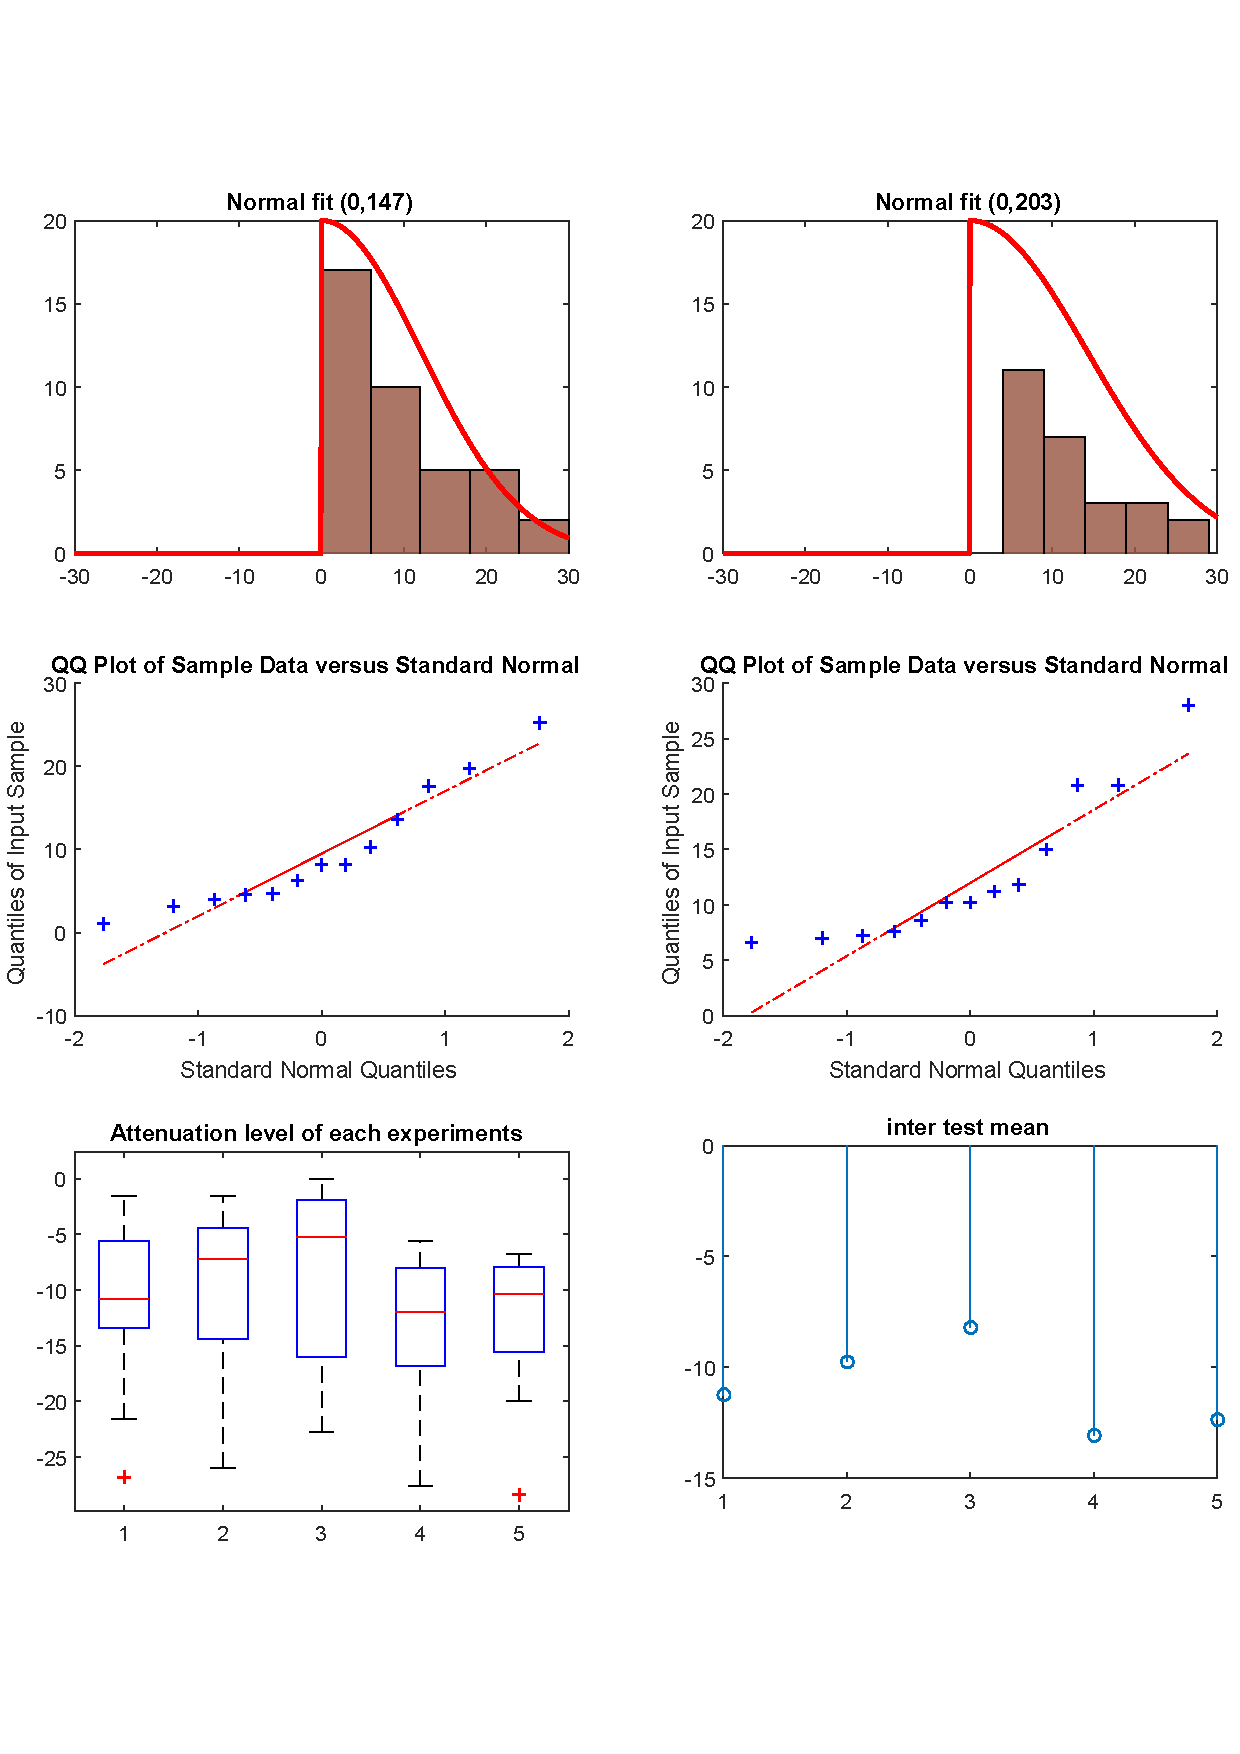
\includegraphics[width=\textwidth]{AttenuationExperiment/figure1.pdf}
\end{figure}


